\section{QuickDough Framework}\label{sec:framework}
QuickDough is a development framework for FPGA-accelerated applications. It generates FPGA accelerators for compute intensive loop kernels rapidly through the use of a pre-built soft coarse-grained reconfigurable array (SCGRA) overlay. It also generates the communication infrastructure between the CPU host and the accelerator automatically, integrating both software and hardware generation in a unified framework. The overall design goal of QuickDough is to enhance the designer's productivity by greatly reducing the hardware generation time. Instead of spending hours on conventional hardware implementation tools, QuickDough is capable of producing the targeted hardware-software system in the order of seconds. By doing so, it provides a rapid development experience that is compatible with that expected by most software programmers.

To achieve this compilation speed, while maintaining a reasonable accelerator performance, QuickDough avoids the creation of custom hardware directly for each application. Instead, the compute kernel loop bodies are scheduled to execute on an SCGRA overlay based accelerator, which is selected from a pre-built library. By sidestepping the time-consuming low-level hardware implementation tool flow, the time to implementing an accelerator in QuickDough is reduced to essentially just the time spent on accelerator selection and scheduling compute operations on the resulting overlay based accelerator. 

\subsection{QuickDough Overview}
\figref{fig:framework} summarizes the hardware-software compilation flow of QuickDough. Users begin by specifying the regions for accelerations in the form of compute intensive loops. Once a loop is identified, it is further compiled to an SCGRA overlay based FPGA accelerator while the rest part of the program is compiled to the processor through a conventional software compilation.

\begin{figure}[bt]
\vspace{-1em}
    \center{\includegraphics[width=0.95\linewidth]{framework}}
    \caption{QuickDough: FPGA loop accelerator design framework using pre-built accelerator library. 
        The compute intensive loop kernel of an application is compiled to the FPGA accelerator while the rest is compiled to the host processor.}
    \label{fig:framework}
\vspace{-1em}
\end{figure}

The focus of QuickDough is to rapidly generate the FPGA loop accelerator. As QuickDough takes an SCGRA overlay as the backbone of the resulting accelerator, the loop accelerator generation is essentially mapping the high level loop kernel to the SCGRA overlay. To that end, the loop kernel is statically transformed to the corresponding data flow graph (DFG) with user-specified loop unrolling factor. Then the accelerator selection process selects an accelerator from a pre-built accelerator library based on the scheduling performance and the estimated communication cost. The scheduling performance is obtained from the DFG scheduling process which schedules the generated DFG to the SCGRA overlay included in the selected accelerator while the communication cost is obtained through a CPU-FPGA communication estimation model. After the accelerator selection process, the accelerator drivers can be generated accordingly based on the on-chip buffer size of the selected accelerator. Meanwhile, the selected empty pre-built accelerator bitstream and the corresponding scheduling result are integrated to create the final FPGA accelerator configuration bitstream. This bitstream, in combination with the binary code created in the software compilation process, forms the final application that will be executed on the target CPU-FPGA system.

As shown in \figref{fig:framework}, QuickDough still needs a pre-built SCGRA overlay based accelerator library, which is also a challenge to the designers. To address this challenge, the accelerator library pre-building process is also done automatically for the target high-level loop kernels. Detailed accelerator library pre-building process will be elaborated in next section.

\subsection{SCGRA overlay based FPGA accelerator}
QuickDough utilizes an SCGRA overlay as the backbone of the resulting accelerators. \figref{fig:scgra-accelerator} shows the typical structure of an SCGRA overlay based accelerator. It consists of an array of homogeneous simple processing elements (PEs) connected by a direct network executing synchronously. Each PE computes and forwards data in lock steps, allowing deterministic multi-hop data communication that overlaps with computations. The action of each PE in each cycle is controlled by an instruction ROM that is populated with instructions generated by the design framework. Communication between the accelerator and the host processor is carried through a pair of input/output buffers. Accesses to these I/O buffers from the SCGRA array take place in lock step with the rest of the system. The exact buffer location to be accessed is controlled by the AddrIBuf and AddrOBuf blocks. Both of them are ROM populated with address information generated from the QuickDough compiler.

\begin{figure}[tb]
\vspace{-1em}
    \center{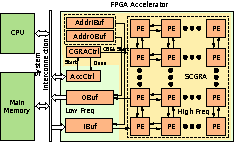
\includegraphics[width=0.65\linewidth]{scgra-accelerator}}
    \caption{SCGRA overlay based FPGA accelerator}
    \label{fig:scgra-accelerator}
\end{figure}

\begin{figure}[tb]
\center{\includegraphics[width=0.7\linewidth]{pe}}
\caption{Fully pipelined PE structure.}
\label{fig:pe}
\end{figure}

\begin{figure}[tb]
\center{\includegraphics[width=0.65\linewidth]{alu}}
\caption{QuickDough ALU supporting up to 16 pipelined 3-input operations.}
\label{fig:ALU}
\vspace{-1em}
\end{figure} 

\subsubsection{PE template}
\figref{fig:pe} shows the current implementation of a QuickDough PE template that features an optional load/store path. At the heart of the PE is an ALU, which is supported by a multi-port data memory and an instruction memory. Three of the data memory's read ports are connected to the ALU as inputs, while the remaining ports are sent to the output multiplexers for connection to neighboring PEs and the optional store path to OBuf external to the PE. At the same time, this data memory takes input from the ALU output, data arriving from neighboring PEs, as well as from the optional IBuf loading path. The action of the PE is controlled by the control words that are read from the instruction memory. Finally, a global signal (\emph{CGRAStart}) from the \emph{SCGRACtrl} block controls the start/stop of all PEs in the array.

\subsubsection{ALU template}
At the heart of the proposed PE is the ALU and it can easily be customized to support different operations specifically for any given user applications. \figref{fig:ALU} shows the ALU template used in the QuickDough overlay. These operators in the ALU may execute concurrently in a pipelined fashion and must complete in a deterministic number of cycles. Given the deterministic nature of the operators, the QuickDough scheduler will ensure that there is no conflict at the output multiplexer.

\subsubsection{Accelerator Controller (\emph{AccCtrl})}
As the accelerator is eventually attached to a processor, it also has a standard accelerator controller AccCtrl to facilitate the HW/SW co-design. Basically, it generates the corresponding triggering signal when the host processor starts the computing and acknowledges the host processor when the computing is done. Most importantly, it also generates cyclic controlling signal that repeats the computing array multiple times which helps to make good use of the communication bandwidth between the main memory and the on-chip buffer. This will be detailed in next subsection. In addition, part of the accelerator controller that is connected to the host processor must handle complex system interconnection protocol and work at lower clock frequency. The other part of the controller that is coupled with the highly pipelined processing array typically work at higher clock frequency. 

\subsection{Loop execution on the accelerator}
The loop kernels are mostly partially unrolled, transformed to DFGs and scheduled to the SCGRA overlays of the accelerators. A straightforward way to perform the whole loop computation on the overlay is to repeat the same DFG computation until the end of the loop. Nevertheless, this may require data transfer between host processor and I/O buffer for each DFG computation. As a result, the communication cost increases dramatically especially when the amount of each data transfer is small. Worse still, input data of the consecutive DFGs may be reused and the straightforward data transfer strategy may greatly increase the total amount of data transfer through out the loop computation. 

To alleviate this problem, we have proposed to batch data transfers for multiple executions of the same DFG into groups as shown in \figref{fig:blocking-and-dfg-gen}. Specifically, after the loop is unrolled $U$ times, $G$ of them are grouped together for each data transfer. This group strategy helps to amortize the initial communication cost between host processor and the accelerator. In addition, it allows input data to be reused for different DFG computation in the same group and the group size is mainly limited by the I/O buffer depth. Meanwhile, the accelerator communicates with host processor for each group execution. The group strategy is also supported by the proposed accelerator micro-architecture as mentioned in previous subsection. Basically, the number of cycles for each DFG execution and the number of the DFG to be iterated in a group should be configured in \emph{AccCtrl}. Finally, the accelerator driver that handles the communication depends on the I/O buffer depth as well. Clearly, accelerator with larger I/O buffer is preferable when the rest part of the accelerator configuration fulfills the requirements. 

\begin{figure}
\vspace{-1em}
\center{\includegraphics[width=0.85\linewidth]{dfg-gen}}
\caption{Loop execution on an SCGRA overlay based FPGA accelerator}
\label{fig:blocking-and-dfg-gen}
\vspace{-1.2em}
\end{figure}

\subsection{FPGA loop accelerator generation}
The aim of QuickDough is to produce FPGA loop accelerator rapidly and thus the loop accelerator generation is the most critical part of QuickDough. It consists of five dependent processes including DFG generation, accelerator selection, DFG scheduling, communication estimation and bitstream integration. They will be detailed in the following sub sections.

\subsubsection{DFG generation}
In order to produce an FPGA loop accelerator using SCGRA overlay, DFGs are extracted from the kernel that is often expressed as inner loop body. In order to transform the loop body to a DFG, data dependency in the loop body must be known at compilation time. Similar to LLVM intermediate representation, simple branches in the loop body can be removed by using PHI instruction which can further be mapped to PHI operation in ALU. The users may further unroll the loops multiple times to increase the amount of operation parallelism in the generated DFG. In this work, we have developed a C++ library to help automate the DFG generation with specified loop unrolling factor.

\subsubsection{DFG Scheduling}
The operations from the user DFG are scheduled to execute on the reconfigurable array. Since the processing elements in the QuickDough overlay execute in lock steps with deterministic latencies, a classical list scheduling algorithm \cite{schutten1996list} was adopted. The challenge in this scheduler is that data communication among the processing elements must be carried out via multi-hop routing in the array. As a result, while it is desirable to schedule data producers and consumers in nearby processing elements to minimize communication latencies, it is also necessary to utilize as much parallel processing power as possible for sake of load balancing. Building on top of our previous work presented in \cite{lin2012energy}, a scheduling metric considering both load balancing and communication cost was adopted in our current implementation.

 \begin{algorithm}
 \small
 \caption{The QuickDough scheduling algorithm.}
 \label{alg:scheduling}
 \begin{algorithmic}
 \PROCEDURE{ListScheduling}
 \STATE Initialize the operation ready list $L$
 \WHILE {$L$ is not empty}
 \STATE select a PE $p$
 \STATE select an operation $l$
 \STATE OPScheduling($p$, $l$)
 \STATE Update $L$
 \ENDWHILE
 \ENDPROCEDURE
 \STATE
 \PROCEDURE {OPScheduling($p$,$l$)}
 \FORALL {predecessor operations $s$ of $l$}
 \STATE Find nearest PE $q$ that has a copy of operation $s$
 \STATE Find shortest routing path from PE $q$ to PE $p$
 \STATE Move operation $s$ from PE $q$ to PE $p$ along the path
 \ENDFOR
 \STATE Do operation $l$ on PE $p$
 \ENDPROCEDURE

 \end{algorithmic}
 \end{algorithm}

\algref{alg:scheduling} briefly illustrates the scheduling algorithm implemented in QuickDough. Initially, an operation ready list is created to represent all operations that are ready to be scheduled. The next step is to select a PE from the SCGRA and an operation from the ready list using a combined communication and load balance metric. When both the PE and the operation to be scheduled are determined, the \code{OPScheduling} procedure starts. It determines an optimized routing path, moves the source operands to the selected PE along the path, and schedules the selected operation to execute accordingly. After this step, the ready list is updated as the latest scheduling may produce more ready operations. This \code{OPScheduling} procedure is repeated until the ready list is empty. Finally, given the operation schedule, the corresponding control words for each PE and the IO buffer accessing sequence will be produced. These control words will subsequently be used for bitstream generation in the following compilation step.

\subsubsection{Accelerator selection}
Accelerator selection process selects an accelerator from the accelerator library based on the resulting accelerator performance which mainly includes the computation latency and communication latency. The computation latency of the loop kernel can be calculated using \eqnref{eq:comp-lat}. $DFG\_Lat(SCGRA\_Size)$ stands for the number of cycles needed to complete the DFG scheduling and mostly depends on the SCGRA overlay size while $Freq$ stands for the pre-built accelerator implementation frequency. The communication latency can be calculated using \eqnref{eq:comm-lat} where $Trans()$ represents the data transfer latency function of the target platform and $GpIn$ and $GpOut$ represent the amount of data transfer of a group.

\begin{equation} \label{eq:comp-lat}
    \footnotesize
    CompLat = DFG\_per\_Loop \times DFG\_Lat(SCGRA\_Size) / Freq
\vspace{-2em}
\end{equation}

\begin{equation} \label{eq:comm-lat}
    \footnotesize
    CommLat = Gp\_per\_Loop \times (Trans(GpIn) + Trans(GpOut))
\end{equation}

On top of the SCGRA size, the rest design parameters also affect the accelerator selection. However, the influence can be immediately analyzed given the DFG scheduling result. For instance, the instruction memory depth must be larger than or equal to $DFG\_Lat$ which represents the number of control words in each PE. Similarly, data memory capacity requirement of each is also decided via the DFG scheduling. The input/output buffer depth must be larger than or equal to $GpIn$ / $GpOut$. In other words, the maximum grouping factor is decided by the capacity of the I/O buffers. Thus the communication latency is essentially determined by the input/output buffer depth according to \eqnref{eq:comm-lat}.

In summary, the performance of the accelerator can be estimated with the analytical models when the scheduling performance is obtained through the DFG scheduling while the scheduling performance is mostly determined by the SCGRA overlay size. The analytical estimation is fast while the scheduling process is relatively slow. Therefore, the accelerator selection process essentially centers the SCGRA overlay size selection and then explores all the accelerator configurations with the same SCGRA overlay size. 

To compromise the loop accelerator generation time and performance, three different levels of accelerator selection optimization levels are provided in this framework namely O0, O1 and O2 centering the SCGRA overlay size selection.
O0 doesn't provide any optimization, and it selects an accelerator with the smallest SCGRA overlay. O1 estimates three typical accelerators with the smallest SCGRA overlay, a medium one and the largest SCGRA overlay. Then the one that provides the best performance will be adopted. O3 explores all the accelerators in the library and searches for the best accelerator configuration. With the increase of the optimization level, the accelerator selection process spends more efforts in searching the accelerator library for better performance and thus results in longer acceleration generation time.

\subsubsection{Accelerator bitstream generation}
The final step of the accelerator generation is to generate 
the instructions for each PE and the address sequences for the 
I/O buffers based on the scheduling result, which will subsequently 
be incorporated into the configuration bitstream of the overlay produced 
from previous steps. Then we take advantage of the reconfigurability 
of SRAM based FPGAs and store the cycle-by-cycle configuration words 
using on-chip ROMs. The content of the ROMs are embedded in the 
bitstream and the \code{data2mem} tool from Xilinx \cite{data2mem} is 
used to update the ROM content of the pre-built bitstream directly. 
To complete the bitstream integration, \code{BMM} file that describes 
the organization and placements of the ROMs in the overlay is extracted 
from \code{XDL} file corresponding to the overlay implementation \cite{beckhoff2011xilinx}.
This bitstream integration process costs only a few seconds of the compilation time.
